\documentclass[12pt,a4paper]{article}

% Pacotes básicos
\usepackage[utf8]{inputenc}
\usepackage[T1]{fontenc}
\usepackage[brazil]{babel}
\usepackage{setspace}
\usepackage{array}
\usepackage{longtable}
\usepackage{geometry}
\usepackage{xcolor}
\usepackage{ulem}
\usepackage{graphicx}
\usepackage{authblk}
\usepackage{hyperref}



% Configurações
\geometry{margin=2cm}
\setlength{\parskip}{1em}
\setlength{\affilsep}{1em}


\begin{document}

% Título e autores
\title{Organizador De Eventos}
\author{Autores:\\Enrico Minto Spanier - 10419775 \\ Guilherme Vecchi Bonotti Freitas Silveira - 10418517 \\ Alexandre Luppi Severo e Silva - 10419724}
\date{\today}


\maketitle
\tableofcontents
\newpage

\section{Introdução}
O sistema é um aplicativo 100\% gratuito desenvolvido para transformar a forma como você agenda, divulga e gerencia eventos. Mais do que uma simples ferramenta, ele funciona como um hub inteligente que conecta organizadores e participantes, oferecendo recursos práticos para cada etapa do processo desde a criação do evento até o acompanhamento dos resultados.

Com ele, qualquer pessoa pode planejar eventos sem restrições de tamanho ou perfil: de um show de stand-up a uma conferência corporativa para centenas de participantes. A interface é intuitiva, permitindo que até usuários iniciantes configurem suas atividades em poucos minutos, enquanto recursos extras como integração com redes sociais, confirmação de presença e relatórios em tempo real garantem eficiência e alcance máximo.

\section{Requisitos}

\subsection{Requisitos Funcionais}

%inicio tabela

\begin{tabular}{ | m{6em} | m{5cm}| m{20em} |}
  \hline
  Requisitos Funcionais & Nome & Descrição \\
  \hline
  RF-01 & Cadastro de Eventos & O sistema deve permitir que organizadores cadastrem novos eventos, incluindo as informações necessarias \\ 
  \hline
  RF-02 & Inscrição de Participantes & O sistema deve permitir que participantes se inscrevam em eventos disponíveis\\ 
  \hline
  RF-03 & Controle de Vagas & O sistema deve controlar o número de vagas disponíveis por evento, impedindo novas inscrições quando o limite for atingido \\ 
  \hline
  RF-04 & Registro de Eventos & O sistema deve armazenar dados de cada evento \\ 
  \hline
\end{tabular}

%fim tabela

\subsection{Requisitos não Funcionais}

%inicio tabela
\begin{tabular}{ | m{6em} | m{5cm}| m{20em} |}
  \hline
  Requisitos Não Funciomais & Nome & Descrição \\
  \hline
  RNF-01 & Segurança & O sistema deve implementar criptografia para armazenamento de dados \\ 
  \hline
  RNF-02 & Desempenho & O sistema deve ser capaz de suportar até 1.000 acessos simultâneos sem degradação da performance\\ 
  \hline
  RNF-03 & Disponibilidade & O sistema deve estar disponível 24/7 \\ 
  \hline
  RNF-04 & Escalabilidade & A arquitetura deve permitir a adição de novos eventos sem comprometer a performance e segurança \\ 
  \hline
  RNF-05 & Conformidade & O sistema deve atender a padrões de segurança como ISO 27001 e NIST 800-53 para segurança cibernética \\ 
  \hline
  RNF-06 & Usabilidade & A interface do sistema deve ser intuitiva e acessível \\ 
  \hline
\end{tabular}
%fim tabela


\section{Casos de Uso}

\begin{center}
  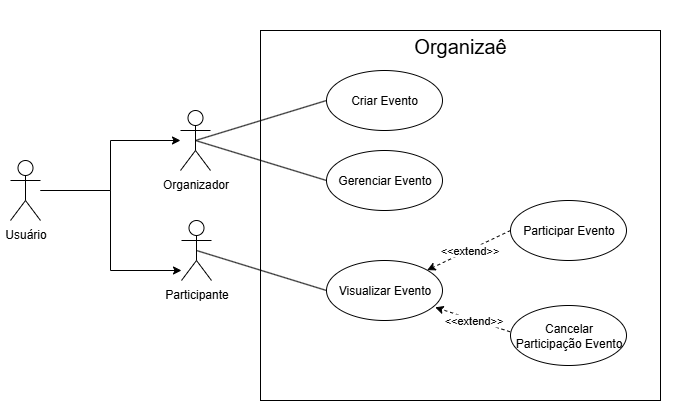
\includegraphics[width=0.8\textwidth]{D_Organizae_drawio.png}
\end{center}

\newpage

\subsection{Caso de Uso: Visualizar Evento}
\begin{longtable}{|p{4cm}|p{11cm}|}
\hline
\textbf{Nome do Caso de Uso} & Visualizar Evento \\ \hline
\textbf{Ator Principal} & Participante \\ \hline
\textbf{Ator Secundário} & Banco de Dados \\ \hline
\textbf{Resumo} & Esse caso de uso descreve as etapas percorridas onde o participante vê uma lista de eventos podendo participar futuramente \\ \hline
\textbf{Pré-Condição} & \\ \hline
\textbf{Pós Condição} & Pode iniciar o Participar Evento ou Cancelar Participação Evento \\ \hline
\textbf{Fluxo Principal} & --- \\ \hline
\textbf{Ações do Ator} & \textbf{Ações do Sistema} \\ \hline
1. Participante entra no Organizaê & 2. Exibe a home page \\ \hline
3. Participante seleciona o evento desejado & 4. Sistema exibe todos os detalhes do evento \\ \hline
5. Participante fecha os detalhes do evento & \\ \hline
\textbf{Fluxo Alternativo} & --- \\ \hline
5a. Participante participa do evento & 6a. Sistema inicia o caso de Participar Evento \\ \hline
\textbf{Fluxo Alternativo} & --- \\ \hline
5b. Participante cancela a participação do evento & 6b. Sistema inicia o caso de Cancelar Participação Evento \\ \hline
\textbf{Fluxo de Exceção} & --- \\ \hline
1. & \\ \hline
& 2. \\ \hline
\textbf{Restrições e Validações:} & \\ \hline
\end{longtable}

\vspace{1cm}

\newpage

\subsection{Caso de Uso: Participar Evento}
\begin{longtable}{|p{4cm}|p{11cm}|}
\hline
\textbf{Nome do Caso de Uso} & Partici
par Evento \\ \hline
\textbf{Ator Principal} & Participante \\ \hline
\textbf{Ator Secundário} & Banco de Dados \\ \hline
\textbf{Resumo} & Esse caso de uso descreve as etapas percorridas onde o participante confirma sua participação em um evento \\ \hline
\textbf{Pré-Condição} & O usuário deve estar logado no sistema \newline O sistema deve estar na página do evento \\ \hline
\textbf{Pós-Condição} & A participação do usuário ao evento é registrada no sistema \\ \hline
\textbf{Fluxo Principal} & --- \\ \hline
\textbf{Ações do Ator} & \textbf{Ações do Sistema} \\ \hline
1. Participante seleciona a opção "Participar" do evento & \\ \hline
& 2. Sistema requisita a confirmação da participação do usuário no evento \\ \hline
3. Participante confirma a participação & \\ \hline
& 4. Sistema registra a participação do usuário no evento \\ \hline
& 5. Sistema exibe mensagem de confirmação de participação \\ \hline
\textbf{Fluxo Alternativo} & --- \\ \hline
& 1a. Sistema identifica que não há login na sessão \\ \hline
& 2a. Sistema redireciona para tela de login \\ \hline
3a. Organizador insere suas credenciais & \\ \hline
& 4a. Sistema valida as credenciais com o banco de dados \\ \hline
\textbf{Fluxo de Exceção} & --- \\ \hline
& 4b. Sistema exibe mensagem de erro no login e solicita nova tentativa \\ \hline
\textbf{Restrições e Validações} & 1. Apenas usuários autenticados podem participar de eventos \newline 2. O sistema deve impedir participação duplicada no mesmo evento \\ \hline
\end{longtable}

\vspace{1cm}

\newpage

\subsection{Caso de Uso: Cancelar Participação Evento}
\begin{longtable}{|p{4cm}|p{11cm}|}
\hline
\textbf{Nome do Caso de Uso} & Cancelar Participação Evento \\ \hline
\textbf{Ator Principal} & Participante \\ \hline
\textbf{Ator Secundário} & Banco de Dados \\ \hline
\textbf{Resumo} & Esse caso de uso descreve as etapas percorridas onde o participante cancela sua participação previamente registrada em um evento \\ \hline
\textbf{Pré-Condição} & O usuário deve estar logado no sistema \newline O usuário deve ser participante no evento \\ \hline
\textbf{Pós-Condição} & A participação do usuário no evento é cancelada do sistema \\ \hline
\textbf{Fluxo Principal} & --- \\ \hline
\textbf{Ações do Ator} & \textbf{Ações do Sistema} \\ \hline
1. Participante seleciona a opção "Cancelar Participação" no evento & \\ \hline
& 2. Sistema verifica se há participação registrada \\ \hline
& 3. Sistema requisita a confirmação do cancelamento da participação do usuário no evento \\ \hline
4. Participante confirma o cancelamento da participação & \\ \hline
& 5. Sistema remove a participação do usuário no evento \\ \hline
& 6. Sistema exibe mensagem de confirmação de cancelamento \\ \hline
\textbf{Fluxo Alternativo} & --- \\ \hline
& 1a. Sistema identifica que não há login na sessão \\ \hline
& 2a. Sistema redireciona para tela de login \\ \hline
3a. Organizador insere suas credenciais & \\ \hline
& 4a. Sistema valida as credenciais com o banco de dados \\ \hline
\textbf{Fluxo de Exceção} & --- \\ \hline
& 4b. Credenciais inválidas \\ \hline
& 5b. Sistema exibe mensagem de erro no login e solicita nova tentativa \\ \hline
\textbf{Fluxo de Exceção} & --- \\ \hline
& 2c. Participante não está participando do evento \\ \hline
& 3c. Sistema exibe mensagem informando que não há participação registrada \\ \hline
\textbf{Fluxo de Exceção} & --- \\ \hline
& 5d. Falha ao cancelar participação \\ \hline
& 6d. Sistema exibe erro e sugere tentar novamente mais tarde \\ \hline
\textbf{Restrições e Validações} & 1. Apenas usuários autenticados podem cancelar participação \newline 2. Cancelamento só é possível se houver uma participação registrada previamente \\ \hline
\end{longtable}

\vspace{1cm}

\subsection{Caso de Uso: Criar Evento}
\begin{longtable}{|p{4cm}|p{11cm}|}
\hline
\textbf{Nome do Caso de Uso} & Criar Evento \\ \hline
\textbf{Ator Principal} & Organizador \\ \hline
\textbf{Ator Secundário} & Banco de Dados \\ \hline
\textbf{Resumo} & Esse caso de uso descreve as etapas percorridas para criar novos eventos \\ \hline
\textbf{Pré-Condição} & Estar logado no sistema Organizaê \\ \hline
\textbf{Pós Condição} & Evento cadastrado no sistema \\ \hline
\textbf{Fluxo Principal} & \\ \hline
\textbf{Ações do Ator} & \textbf{Ações do Sistema} \\ \hline
1. Organizador entra no Organizaê & \\ \hline
2. Organizador seleciona opção de criar evento & \\ \hline
& 3. Sistema exibe a tela de criação de eventos na qual irá solicitar as informações do evento \\ \hline
4. Usuário insere todas as informações necessárias para o evento & \\ \hline
& 5. Sistema atualiza a lista de eventos e volta para a home page \\ \hline
\textbf{Fluxo Alternativo} & --- \\ \hline
& 3a. Sistema identifica que não há login na sessão \\ \hline
& 4a. Sistema redireciona para tela de login \\ \hline
5a. Organizador insere suas credenciais & \\ \hline
& 6a. Sistema valida as credenciais com o banco de dados \\ \hline
\textbf{Fluxo de Exceção} & --- \\ \hline
1. & \\ \hline
& 2. \\ \hline
\textbf{Restrições e Validações:} & 1. Apenas usuários autenticados podem criar eventos \\ \hline
\end{longtable}

\vspace{1cm}

\newpage

\subsection{Caso de Uso: Gerenciar Evento}
\begin{longtable}{|p{4cm}|p{11cm}|}
\hline
\textbf{Nome do Caso de Uso} & Gerenciar Evento \\ \hline
\textbf{Ator Principal} & Organizador \\ \hline
\textbf{Ator Secundário} & Banco de Dados \\ \hline
\textbf{Resumo} & Esse caso de uso descreve as etapas percorridas para criar novos eventos \\ \hline
\textbf{Pré-Condição} & Estar logado no sistema Organizaê \\ \hline
\textbf{Pós Condição} & \\ \hline
\textbf{Fluxo Principal} & \\ \hline
\textbf{Ações do Ator} & \textbf{Ações do Sistema} \\ \hline
1. Organizador entra no Organizaê & \\ \hline
2. Organizador seleciona opção meus eventos & \\ \hline
& 3. Sistema exibe todos os eventos do Organizador \\ \hline
4. Organizador seleciona o evento desejado & \\ \hline
& 5. Sistema exibe as informações sobre o evento selecionado e permite alterações \\ \hline
6. Organizador altera informações desejadas e salva as novas & \\ \hline
& 7. Sistema atualiza a lista de eventos e volta para a home page \\ \hline
\textbf{Fluxo Alternativo} & --- \\ \hline
& 2a. Sistema identifica que não há login na sessão \\ \hline
& 3a. Sistema redireciona para tela de login \\ \hline
4a. Participante insere suas credenciais & \\ \hline
& 5a. Sistema valida as credenciais com o banco de dados \\ \hline
6b. Organizador opta por excluir o evento & \\ \hline
& 7b. Sistema requisita a confirmação da exclusão do evento \\ \hline
8b. Organizador confirma a exclusão & \\ \hline
& 9b. Sistema remove o evento da lista de eventos \\ \hline
\textbf{Fluxo de Exceção} & --- \\ \hline
1. & \\ \hline
& 2. \\ \hline

\textbf{Restrições e Validações:} & 1. Apenas organizadores autenticados podem editar eventos 
\newline 2. Apenas o organizador que criou o evento pode gerenciá-lo \\ \hline
\end{longtable}

\section{Diagrama de Sequencia}

\subsection{Caso de Uso Criar Evento}
 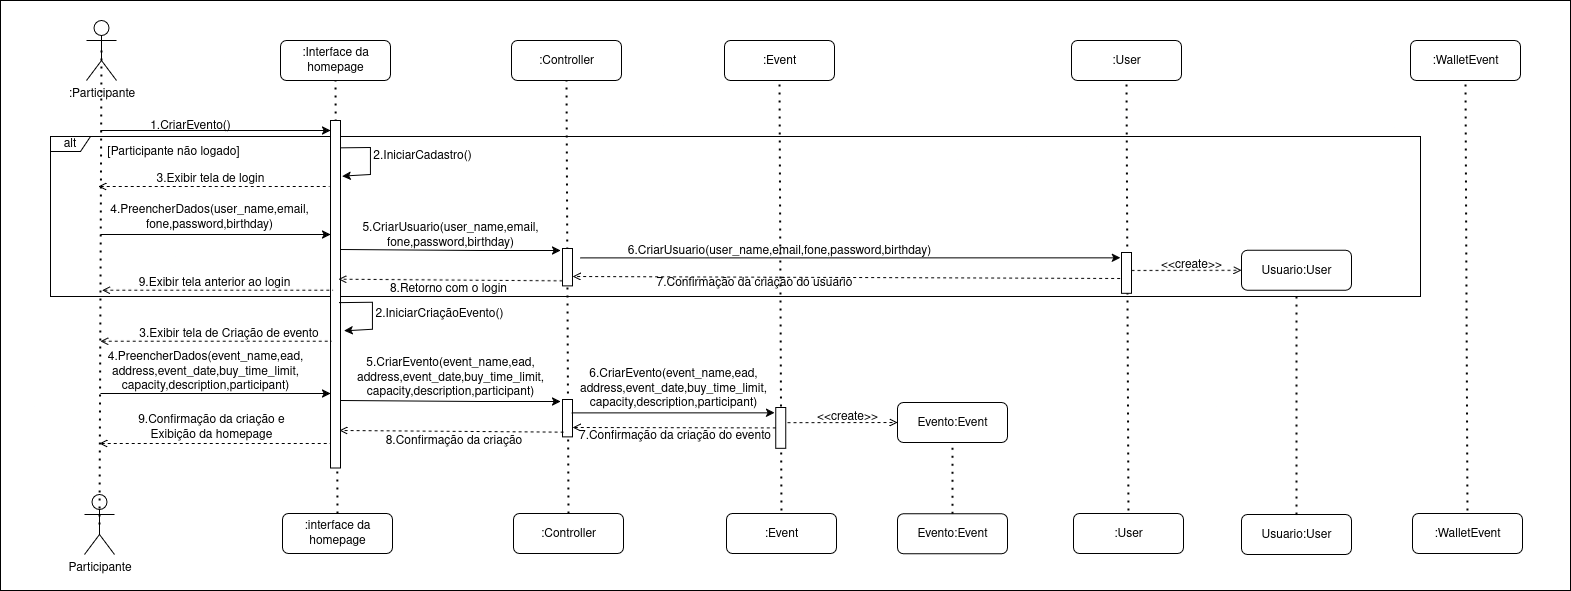
\includegraphics[width=1\textwidth]{Diagrama_Criar.png}

\subsection{Caso de Uso Gerenciar Evento}
 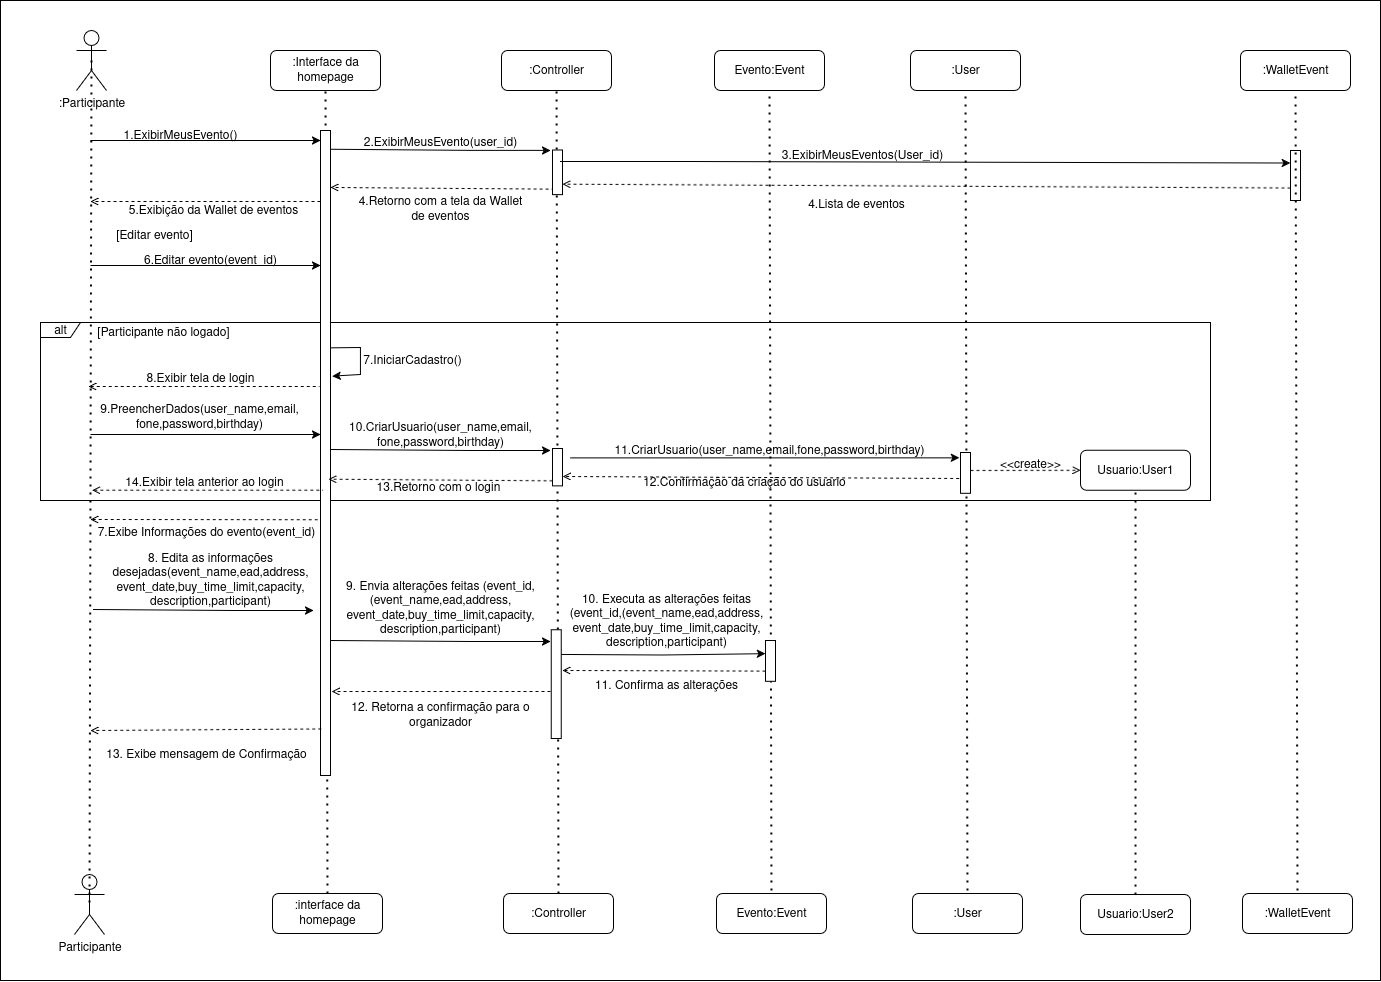
\includegraphics[width=1\textwidth]{Diagrama_Editar.png}


\subsection{Casos de Uso: Visualizar, Participar e Cancelar participação}
 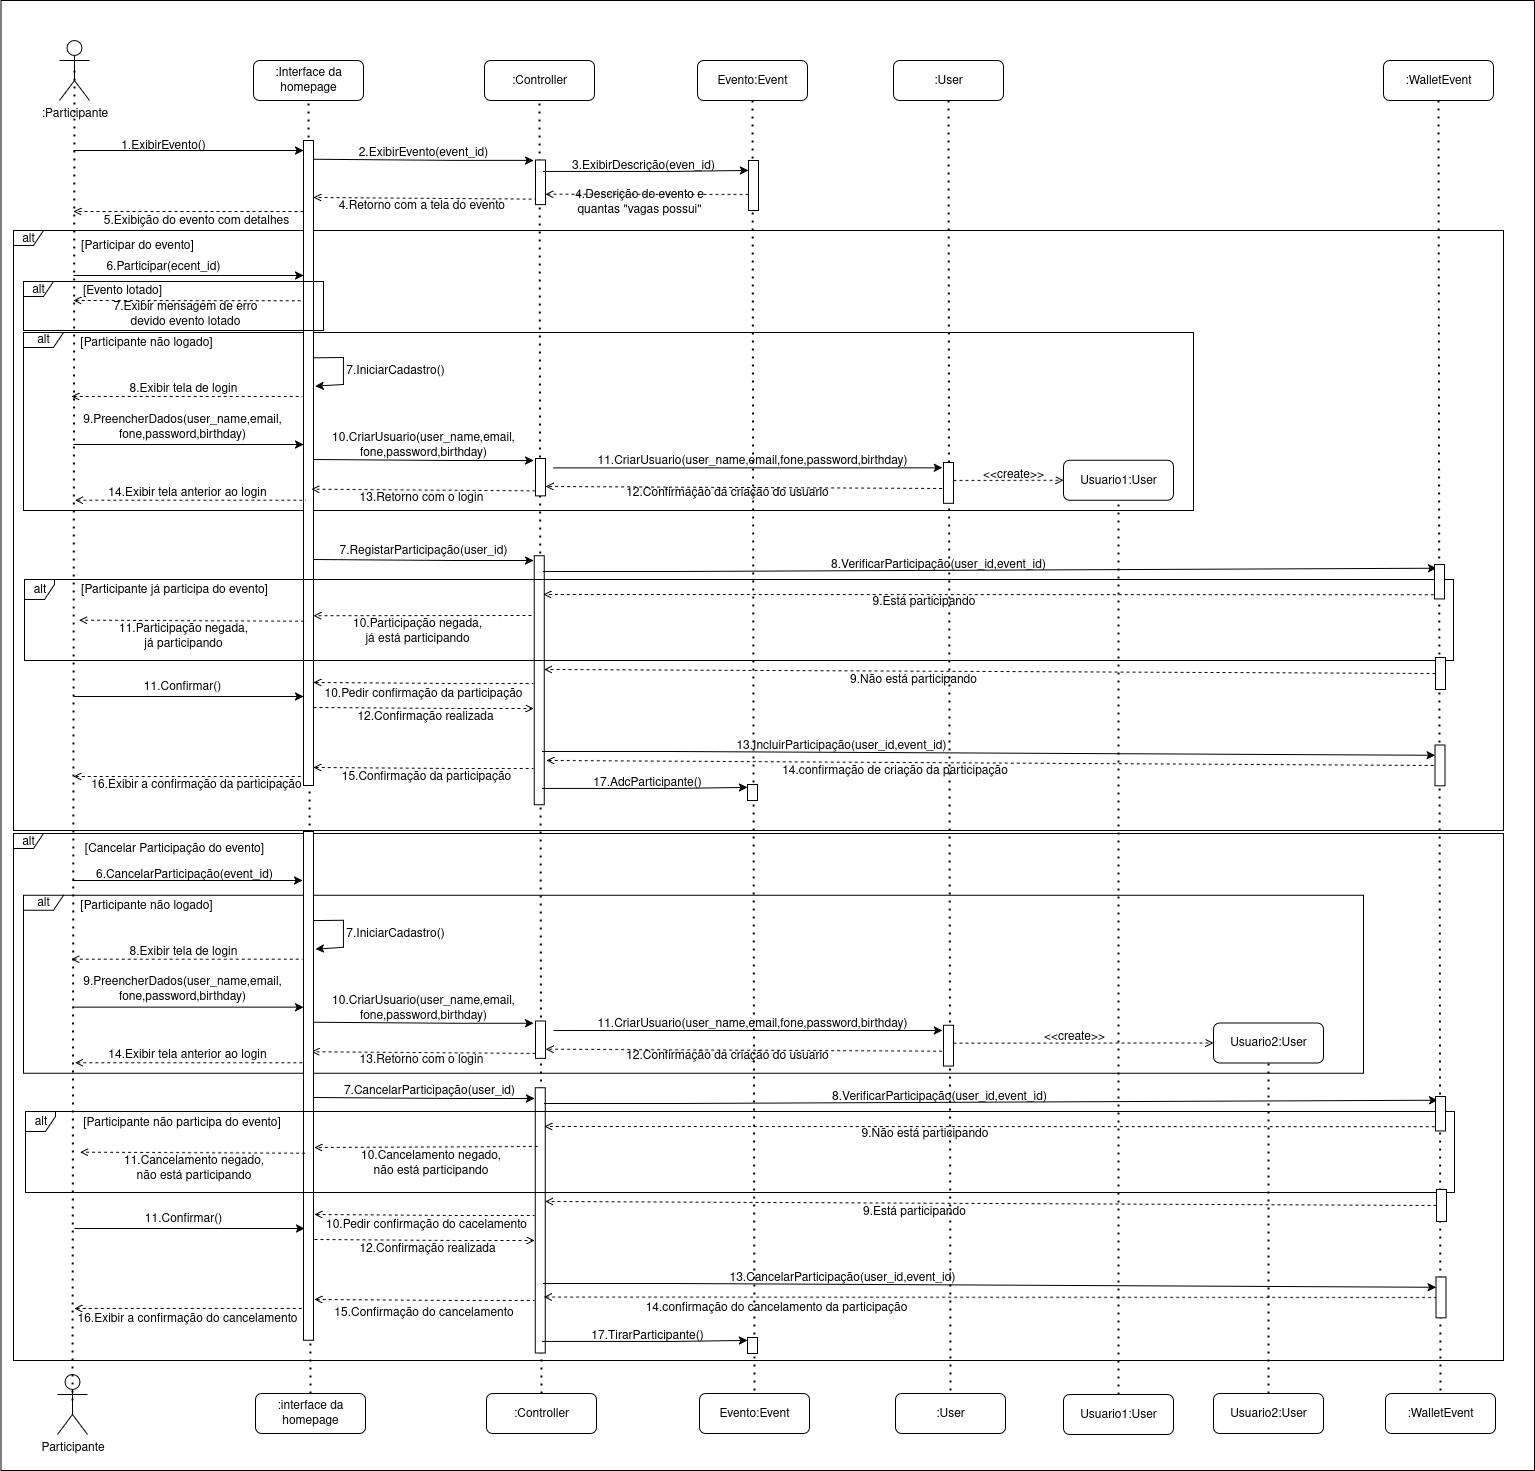
\includegraphics[width=1\textwidth]{Diagrama_3_em_1.png}

\section{Link Prototipação}
\href{https://www.figma.com/design/hQo4WzJU1nHs5j3TelntQZ/Sem-t%C3%ADtulo?node-id=0-1&p=f}{\color{blue}\uline{Link do Figma}}


\section{Bibliográfia}

\subsection{Imagens}
\sloppy
link: https://airsoftrs.com/05-06-2022-operacao-comando-selva-tabai-rs/ \\
link: https://www.sympla.com.br/evento/1-confraternizacao-airsoft-amazonense/978578?referrer=www.google.com \\
link: https://airsoftrs.com/24-03-2024-operacao-maremoto-milsim-santiago-rs/ \\
link: https://airsoftzone.com.br/evento/158 \\
link: https://airsoftrs.com/cobertura-da-operacao-troia-3-em-vacaria-rs/ \\
link: https://jornalceleiro.com.br/2022/12/equipe-hard-de-airsoft-realiza-mega-evento-no-parana-e-deseja-repetir-o-feito-em-campos-novos \\

\end{document}
